\documentclass[aspectratio=169]{beamer}
\usepackage{booktabs}
\usepackage{pgfplots}
\pgfplotsset{compat=1.18}
\usepackage{tikz}
\usetikzlibrary{shapes.geometric,arrows.meta,positioning,fit,backgrounds,calc,decorations.pathreplacing}
\usepackage{xcolor}
\usepackage{colortbl}
\usepackage{multirow}
\usepackage{array}
\usepackage{fontawesome5}
\usepackage{amsmath}

% Company colors
\definecolor{TIRed}{RGB}{199,0,57}
\definecolor{ADIBlue}{RGB}{0,100,175}
\definecolor{NXPOrange}{RGB}{255,102,0}
\definecolor{DarkGray}{RGB}{50,50,50}
\definecolor{LightGray}{RGB}{240,240,240}
\definecolor{AccentGreen}{RGB}{0,150,80}
\definecolor{AccentPurple}{RGB}{120,0,180}

\usetheme{Madrid}
\usecolortheme[named=DarkGray]{structure}
\setbeamercolor{title}{fg=white,bg=DarkGray}
\setbeamercolor{frametitle}{fg=white,bg=DarkGray}
\setbeamercolor{block title}{fg=white,bg=DarkGray}
\setbeamerfont{title}{size=\Large,series=\bfseries}
\setbeamerfont{frametitle}{size=\normalsize,series=\bfseries}
\setbeamertemplate{navigation symbols}{}
\setbeamertemplate{footline}[frame number]

% Colored company boxes
\newcommand{\tibox}[1]{\colorbox{TIRed!15}{\textcolor{TIRed}{\textbf{#1}}}}
\newcommand{\adibox}[1]{\colorbox{ADIBlue!15}{\textcolor{ADIBlue}{\textbf{#1}}}}
\newcommand{\nxpbox}[1]{\colorbox{NXPOrange!15}{\textcolor{NXPOrange}{\textbf{#1}}}}

\title{Edge AI Model Zoo\\Cross-Company Comparison}
\subtitle{TI EdgeAI \textbullet\ ADI AI8X \textbullet\ NXP eIQ}
\author{ModelZooDecks Analysis}
\date{August 2026}
\institute{Edge AI Platform Evaluation}

\begin{document}

% -------------------------------------------------
\begin{frame}
\titlepage
\end{frame}

% -------------------------------------------------
\begin{frame}{Agenda}
\tableofcontents
\end{frame}

% ================================================
\section{Platform Overview}
% ================================================

\begin{frame}{Three Edge AI Ecosystems}
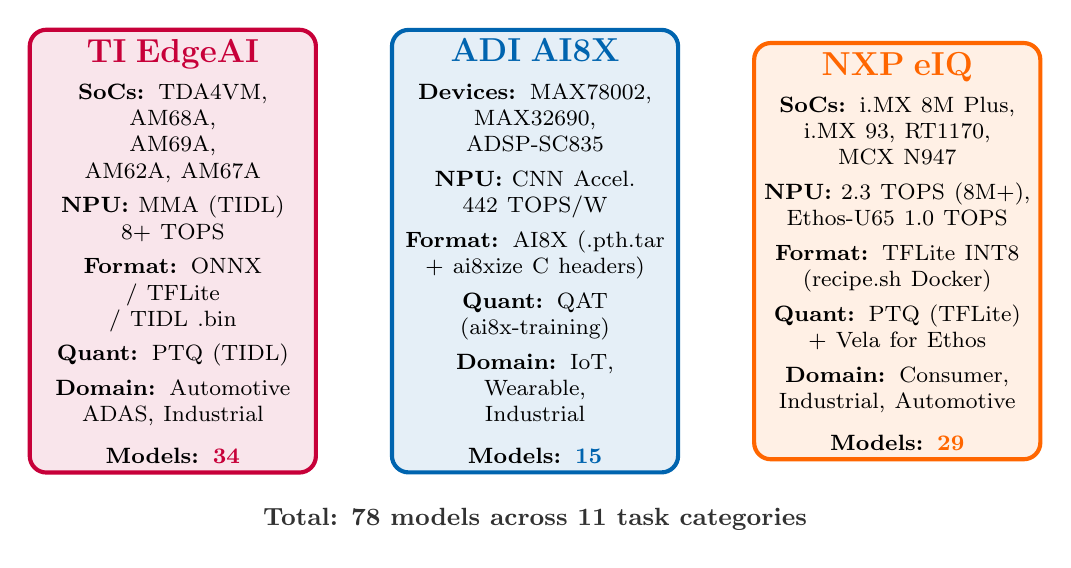
\begin{tikzpicture}[remember picture]
  % TI box
  \node[draw=TIRed,fill=TIRed!10,rounded corners=6pt,minimum width=3.6cm,minimum height=5.2cm,
        text width=3.4cm,align=center,line width=1.5pt] (ti) at (0,0) {
    \textcolor{TIRed}{\textbf{\large TI EdgeAI}}\\[4pt]
    \footnotesize
    \textbf{SoCs:} TDA4VM, AM68A,\\AM69A, AM62A, AM67A\\[3pt]
    \textbf{NPU:} MMA (TIDL)\\8+ TOPS\\[3pt]
    \textbf{Format:} ONNX / TFLite\\/ TIDL .bin\\[3pt]
    \textbf{Quant:} PTQ (TIDL)\\[3pt]
    \textbf{Domain:} Automotive\\ADAS, Industrial\\[3pt]
    \textbf{Models:} \textcolor{TIRed}{\textbf{34}}
  };
  % ADI box
  \node[draw=ADIBlue,fill=ADIBlue!10,rounded corners=6pt,minimum width=3.6cm,minimum height=5.2cm,
        text width=3.4cm,align=center,line width=1.5pt] (adi) at (4.6,0) {
    \textcolor{ADIBlue}{\textbf{\large ADI AI8X}}\\[4pt]
    \footnotesize
    \textbf{Devices:} MAX78002,\\MAX32690, ADSP-SC835\\[3pt]
    \textbf{NPU:} CNN Accel.\\442 TOPS/W\\[3pt]
    \textbf{Format:} AI8X (.pth.tar\\+ ai8xize C headers)\\[3pt]
    \textbf{Quant:} QAT (ai8x-training)\\[3pt]
    \textbf{Domain:} IoT, Wearable,\\Industrial\\[3pt]
    \textbf{Models:} \textcolor{ADIBlue}{\textbf{15}}
  };
  % NXP box
  \node[draw=NXPOrange,fill=NXPOrange!10,rounded corners=6pt,minimum width=3.6cm,minimum height=5.2cm,
        text width=3.4cm,align=center,line width=1.5pt] (nxp) at (9.2,0) {
    \textcolor{NXPOrange}{\textbf{\large NXP eIQ}}\\[4pt]
    \footnotesize
    \textbf{SoCs:} i.MX 8M Plus,\\i.MX 93, RT1170, MCX N947\\[3pt]
    \textbf{NPU:} 2.3 TOPS (8M+),\\Ethos-U65 1.0 TOPS\\[3pt]
    \textbf{Format:} TFLite INT8\\(recipe.sh Docker)\\[3pt]
    \textbf{Quant:} PTQ (TFLite)\\+ Vela for Ethos\\[3pt]
    \textbf{Domain:} Consumer,\\Industrial, Automotive\\[3pt]
    \textbf{Models:} \textcolor{NXPOrange}{\textbf{29}}
  };
  % Total label
  \node[below=0.3cm of ti.south,xshift=4.6cm,font=\small\bfseries,text=DarkGray]
    {Total: \textbf{78 models} across 11 task categories};
\end{tikzpicture}
\end{frame}

% -------------------------------------------------
\begin{frame}{Hardware Spectrum: From mW to 30W}
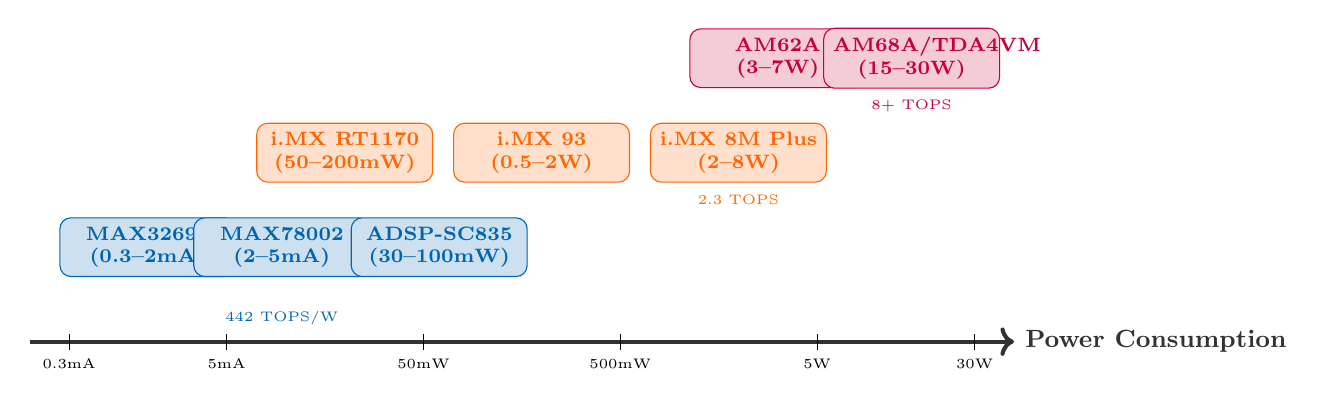
\begin{tikzpicture}
  % Power axis
  \draw[->,line width=1.5pt,color=DarkGray] (0,0) -- (12.5,0)
    node[right,font=\small\bfseries] {Power Consumption};
  % Power labels
  \foreach \x/\lbl in {0.5/0.3mA,2.5/5mA,5/50mW,7.5/500mW,10/5W,12/30W}
    \draw (\x,0.1) -- (\x,-0.1) node[below,font=\tiny] {\lbl};
  % ADI devices
  \node[draw=ADIBlue,fill=ADIBlue!20,rounded corners,font=\scriptsize\bfseries,
        text=ADIBlue,minimum height=0.7cm,text width=2cm,align=center]
    at (1.5,1.2) {MAX32690\\(0.3--2mA)};
  \node[draw=ADIBlue,fill=ADIBlue!20,rounded corners,font=\scriptsize\bfseries,
        text=ADIBlue,minimum height=0.7cm,text width=2cm,align=center]
    at (3.2,1.2) {MAX78002\\(2--5mA)};
  \node[draw=ADIBlue,fill=ADIBlue!20,rounded corners,font=\scriptsize\bfseries,
        text=ADIBlue,minimum height=0.7cm,text width=2cm,align=center]
    at (5.2,1.2) {ADSP-SC835\\(30--100mW)};
  % NXP devices
  \node[draw=NXPOrange,fill=NXPOrange!20,rounded corners,font=\scriptsize\bfseries,
        text=NXPOrange,minimum height=0.7cm,text width=2cm,align=center]
    at (4.0,2.4) {i.MX RT1170\\(50--200mW)};
  \node[draw=NXPOrange,fill=NXPOrange!20,rounded corners,font=\scriptsize\bfseries,
        text=NXPOrange,minimum height=0.7cm,text width=2cm,align=center]
    at (6.5,2.4) {i.MX 93\\(0.5--2W)};
  \node[draw=NXPOrange,fill=NXPOrange!20,rounded corners,font=\scriptsize\bfseries,
        text=NXPOrange,minimum height=0.7cm,text width=2cm,align=center]
    at (9.0,2.4) {i.MX 8M Plus\\(2--8W)};
  % TI devices
  \node[draw=TIRed,fill=TIRed!20,rounded corners,font=\scriptsize\bfseries,
        text=TIRed,minimum height=0.7cm,text width=2cm,align=center]
    at (9.5,3.6) {AM62A\\(3--7W)};
  \node[draw=TIRed,fill=TIRed!20,rounded corners,font=\scriptsize\bfseries,
        text=TIRed,minimum height=0.7cm,text width=2cm,align=center]
    at (11.2,3.6) {AM68A/TDA4VM\\(15--30W)};
  % TOPS annotations
  \node[font=\tiny,text=ADIBlue] at (3.2,0.3) {442 TOPS/W};
  \node[font=\tiny,text=NXPOrange] at (9.0,1.8) {2.3 TOPS};
  \node[font=\tiny,text=TIRed] at (11.2,3.0) {8+ TOPS};
\end{tikzpicture}
\end{frame}

% ================================================
\section{Model Inventory}
% ================================================

\begin{frame}{Model Task Coverage by Company}
\begin{columns}
\column{0.55\textwidth}
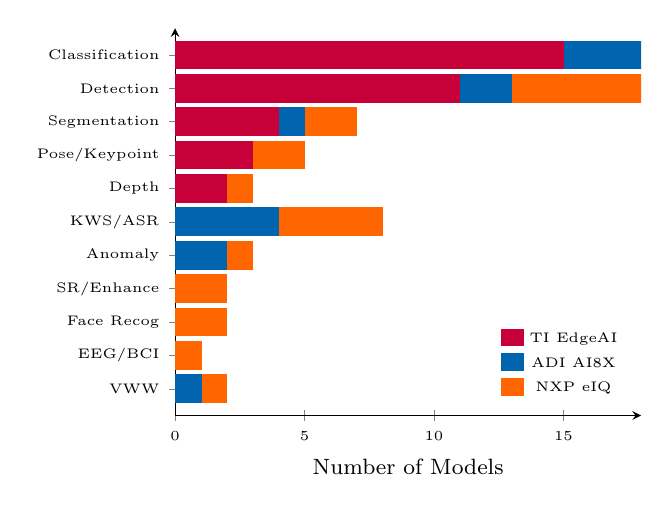
\begin{tikzpicture}
\begin{axis}[
  xbar stacked,
  width=7.5cm, height=6.5cm,
  bar width=10pt,
  xlabel={\footnotesize Number of Models},
  ytick=data,
  yticklabels={
    Classification,Detection,Segmentation,
    Pose/Keypoint,Depth,KWS/ASR,
    Anomaly,SR/Enhance,Face Recog,EEG/BCI,VWW
  },
  yticklabel style={font=\tiny},
  xticklabel style={font=\tiny},
  xlabel style={font=\tiny},
  legend style={font=\tiny,at={(0.98,0.02)},anchor=south east,
                legend columns=1,draw=none},
  xmin=0, xmax=18,
  tick align=inside,
  axis lines=left,
  enlarge y limits=0.08,
]
% TI
\addplot+[xbar,fill=TIRed,draw=TIRed] coordinates {
  (15,10)(11,9)(4,8)(3,7)(2,6)(0,5)(0,4)(0,3)(0,2)(0,1)(0,0)};
% ADI
\addplot+[xbar,fill=ADIBlue,draw=ADIBlue] coordinates {
  (4,10)(2,9)(1,8)(0,7)(0,6)(4,5)(2,4)(0,3)(0,2)(0,1)(1,0)};
% NXP
\addplot+[xbar,fill=NXPOrange,draw=NXPOrange] coordinates {
  (9,10)(7,9)(2,8)(2,7)(1,6)(4,5)(1,4)(2,3)(2,2)(1,1)(1,0)};
\legend{TI EdgeAI,ADI AI8X,NXP eIQ}
\end{axis}
\end{tikzpicture}
\column{0.42\textwidth}
\small
\begin{block}{Key Observations}
\begin{itemize}
  \item \textcolor{TIRed}{\textbf{TI}} leads in vision breadth\\(34 models, pure vision)
  \item \textcolor{ADIBlue}{\textbf{ADI}} leads in power efficiency\\and QAT quality
  \item \textcolor{NXPOrange}{\textbf{NXP}} has most diverse\\task coverage (11 categories)
  \item Only \textcolor{NXPOrange}{\textbf{NXP}} has SR, BCI, face\\recognition
  \item Only \textcolor{TIRed}{\textbf{TI}} + \textcolor{NXPOrange}{\textbf{NXP}} have\\depth estimation
\end{itemize}
\end{block}
\vspace{0.3cm}
\footnotesize
\begin{tabular}{lccc}
\toprule
\textbf{Total} & \textcolor{TIRed}{\textbf{34}} & \textcolor{ADIBlue}{\textbf{15}} & \textcolor{NXPOrange}{\textbf{29}}\\
Audio & 0 & 4 & 4\\
Unique & ADAS & Ultra-LP & SR+BCI\\
\bottomrule
\end{tabular}
\end{columns}
\end{frame}

% ================================================
\section{Classification Models}
% ================================================

\begin{frame}{ImageNet Classification --- Accuracy Comparison}
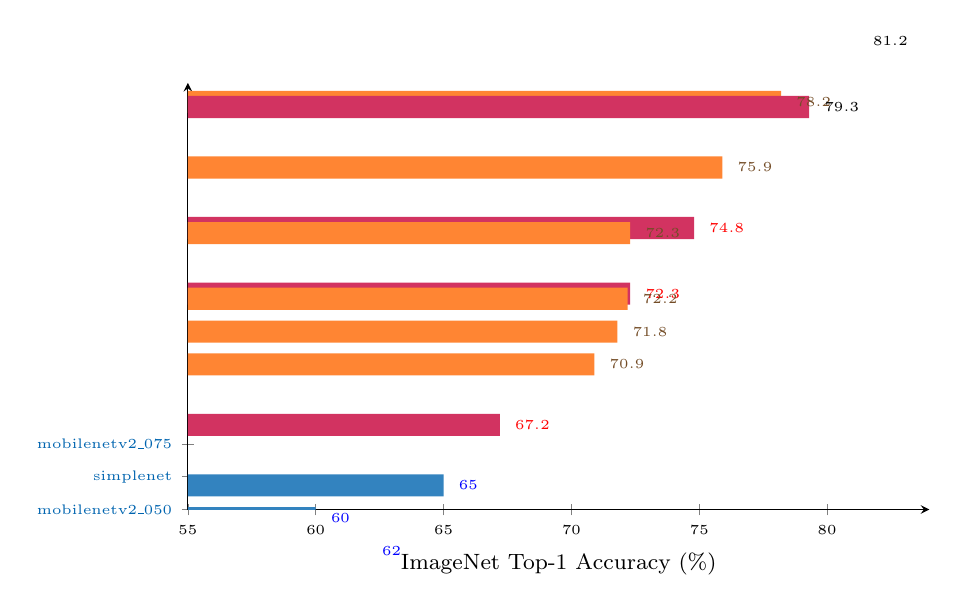
\begin{tikzpicture}
\begin{axis}[
  xbar,
  width=11cm, height=7cm,
  bar width=8pt,
  xlabel={\footnotesize ImageNet Top-1 Accuracy (\%)},
  ytick=data,
  yticklabels={
    \textcolor{ADIBlue}{mobilenetv2\_050},
    \textcolor{ADIBlue}{simplenet},
    \textcolor{ADIBlue}{mobilenetv2\_075},
    \textcolor{TIRed}{mobilenet\_v3\_small},
    \textcolor{NXPOrange}{mobilenetv1},
    \textcolor{NXPOrange}{mobilenetv2},
    \textcolor{NXPOrange}{efficientnet\_lite},
    \textcolor{TIRed}{mobilenet\_v2\_lite},
    \textcolor{NXPOrange}{mnasnet},
    \textcolor{TIRed}{mobilenet\_v3\_large\_lite},
    \textcolor{NXPOrange}{resnet50},
    \textcolor{TIRed}{fastvit\_s12},
    \textcolor{NXPOrange}{inceptionv4},
    \textcolor{TIRed}{swin\_tiny}
  },
  yticklabel style={font=\tiny},
  xticklabel style={font=\tiny},
  xlabel style={font=\tiny},
  xmin=55, xmax=84,
  tick align=inside,
  axis lines=left,
  nodes near coords,
  nodes near coords style={font=\tiny,xshift=2pt},
  every node near coord/.append style={/pgf/number format/.cd,fixed,precision=1},
]
\addplot+[xbar,fill=ADIBlue!80,draw=none] coordinates {(62,0)(60,1)(65,2)};
\addplot+[xbar,fill=TIRed!80,draw=none] coordinates {(67.2,3)(72.3,7)(74.8,9)};
\addplot+[xbar,fill=NXPOrange!80,draw=none] coordinates {(70.9,4)(71.8,5)(72.2,6)(72.3,8)(75.9,10)(78.2,12)};
\addplot+[xbar,fill=TIRed!80,draw=none] coordinates {(79.3,11)(81.2,13)};
\end{axis}
\end{tikzpicture}
\end{frame}

% -------------------------------------------------
\begin{frame}{Classification: Accuracy vs.\ Complexity Tradeoff}
\begin{columns}
\column{0.55\textwidth}
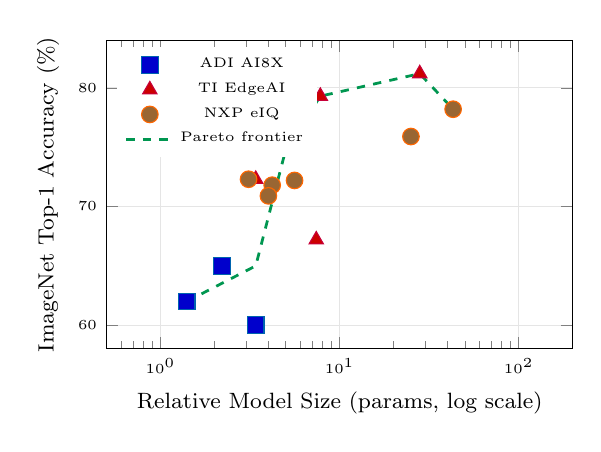
\begin{tikzpicture}
\begin{axis}[
  width=7.5cm, height=5.5cm,
  xlabel={\footnotesize Relative Model Size (params, log scale)},
  ylabel={\footnotesize ImageNet Top-1 Accuracy (\%)},
  xmode=log,
  xmin=0.5, xmax=200,
  ymin=58, ymax=84,
  grid=major,
  grid style={gray!20},
  legend style={font=\tiny,at={(0.02,0.98)},anchor=north west,draw=none},
  xlabel style={font=\tiny},
  ylabel style={font=\tiny},
  xticklabel style={font=\tiny},
  yticklabel style={font=\tiny},
]
\addplot+[only marks,mark=square*,mark size=3pt,color=ADIBlue]
  coordinates {(1.4,62)(2.2,65)(3.4,60)};
\addlegendentry{ADI AI8X}
\addplot+[only marks,mark=triangle*,mark size=3pt,color=TIRed]
  coordinates {(3.4,72.3)(5.0,74.8)(28,81.2)(7.8,79.3)(7.4,67.2)};
\addlegendentry{TI EdgeAI}
\addplot+[only marks,mark=*,mark size=3pt,color=NXPOrange]
  coordinates {(4.2,71.8)(25,75.9)(5.6,72.2)(4.0,70.9)(43,78.2)(3.1,72.3)};
\addlegendentry{NXP eIQ}
\addplot+[no marks,dashed,color=AccentGreen,line width=1pt]
  coordinates {(1.4,62)(3.4,65)(5.0,74.8)(7.8,79.3)(28,81.2)(43,78.2)};
\addlegendentry{Pareto frontier}
\end{axis}
\end{tikzpicture}
\column{0.42\textwidth}
\footnotesize
\begin{block}{Pareto Analysis}
\begin{itemize}
  \item \textcolor{TIRed}{\textbf{Swin-Tiny}} (81.2\%) tops accuracy at moderate size
  \item \textcolor{TIRed}{\textbf{FastViT-S12}} (79.3\%) best accuracy/param on TI
  \item \textcolor{NXPOrange}{\textbf{MobileNetV2}} (71.8\%) optimal for constrained NXP MCUs
  \item \textcolor{ADIBlue}{\textbf{ADI}} models are smallest but lowest accuracy due to hardware op-set limits
\end{itemize}
\end{block}
\begin{alertblock}{Key Tradeoff}
\textbf{+14\% accuracy} from smallest (ADI mobilenetv2\_050 62\%) to largest (TI swin\_tiny 81.2\%) at \textbf{20$\times$ parameter cost}
\end{alertblock}
\end{columns}
\end{frame}

% ================================================
\section{Detection Models}
% ================================================

\begin{frame}{Object Detection --- mAP Comparison (COCO/VOC)}
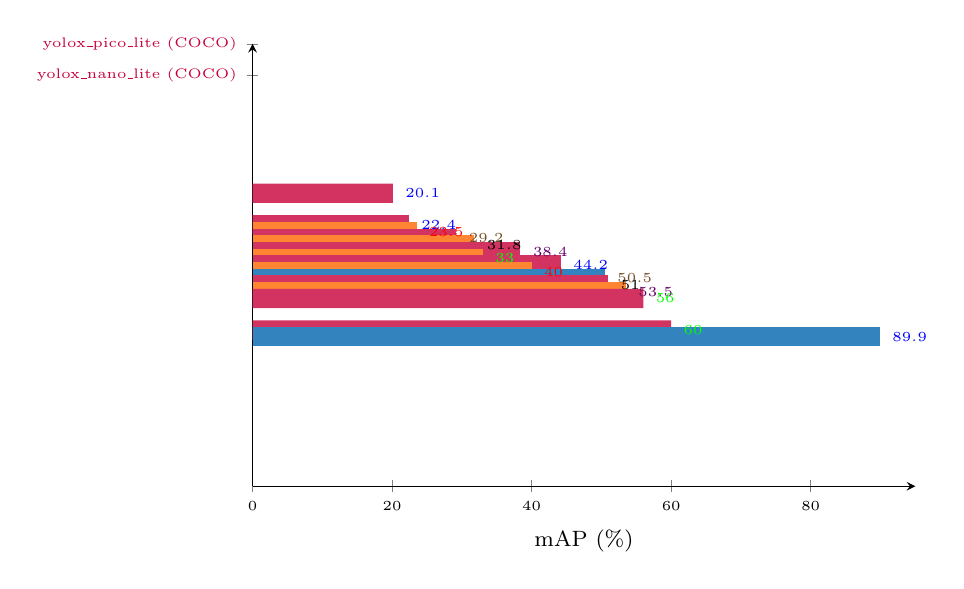
\begin{tikzpicture}
\begin{axis}[
  xbar,
  width=10cm, height=7.2cm,
  bar width=7pt,
  xlabel={\footnotesize mAP (\%)},
  ytick=data,
  yticklabels={
    \textcolor{TIRed}{yolox\_pico\_lite (COCO)},
    \textcolor{TIRed}{yolox\_nano\_lite (COCO)},
    \textcolor{NXPOrange}{nanodet\_m (COCO)},
    \textcolor{TIRed}{yolox\_tiny\_lite (COCO)},
    \textcolor{NXPOrange}{ssdlite\_mobilenetv2 (COCO)},
    \textcolor{TIRed}{yolox\_s\_lite (COCO)},
    \textcolor{NXPOrange}{efficientdet\_lite0 (COCO)},
    \textcolor{TIRed}{yolox\_m\_lite (COCO)},
    \textcolor{NXPOrange}{yolov5 (COCO)},
    \textcolor{ADIBlue}{feature\_pyramid\_net (VOC)},
    \textcolor{TIRed}{yolov7\_l\_lite (COCO)},
    \textcolor{NXPOrange}{yolov8\_m (COCO)},
    \textcolor{TIRed}{rtmdet\_m\_lite (COCO)},
    \textcolor{TIRed}{rtmdet\_l\_lite (COCO)},
    \textcolor{ADIBlue}{tinierssd (QR keypts)}
  },
  yticklabel style={font=\tiny},
  xticklabel style={font=\tiny},
  xmin=0, xmax=95,
  tick align=inside,
  axis lines=left,
  nodes near coords,
  nodes near coords style={font=\tiny,xshift=1pt},
]
\addplot+[xbar,fill=TIRed!80,draw=none] coordinates {(20.1,14)(22.4,13)};
\addplot+[xbar,fill=NXPOrange!80,draw=none] coordinates {(23.5,12)};
\addplot+[xbar,fill=TIRed!80,draw=none] coordinates {(29.2,11)};
\addplot+[xbar,fill=NXPOrange!80,draw=none] coordinates {(31.8,10)};
\addplot+[xbar,fill=TIRed!80,draw=none] coordinates {(38.4,9)};
\addplot+[xbar,fill=NXPOrange!80,draw=none] coordinates {(33.0,8)};
\addplot+[xbar,fill=TIRed!80,draw=none] coordinates {(44.2,7)};
\addplot+[xbar,fill=NXPOrange!80,draw=none] coordinates {(40.0,6)};
\addplot+[xbar,fill=ADIBlue!80,draw=none] coordinates {(50.5,5)};
\addplot+[xbar,fill=TIRed!80,draw=none] coordinates {(51.0,4)};
\addplot+[xbar,fill=NXPOrange!80,draw=none] coordinates {(53.5,3)};
\addplot+[xbar,fill=TIRed!80,draw=none] coordinates {(56.0,2)(60.0,1)};
\addplot+[xbar,fill=ADIBlue!80,draw=none] coordinates {(89.9,0)};
\end{axis}
\end{tikzpicture}
\end{frame}

% -------------------------------------------------
\begin{frame}{Detection: Latency vs.\ mAP Frontier}
\begin{columns}
\column{0.58\textwidth}
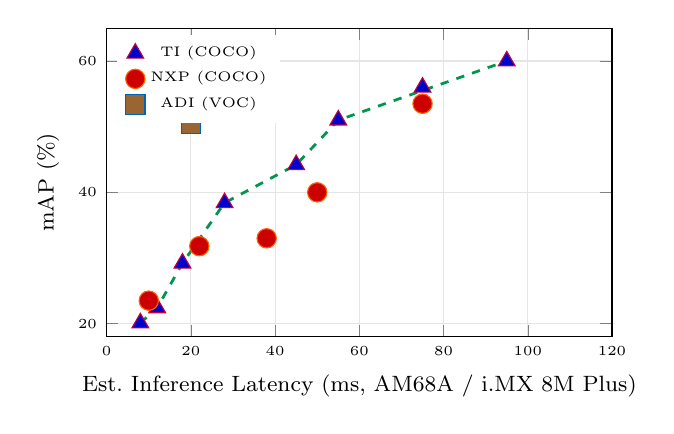
\begin{tikzpicture}
\begin{axis}[
  width=8cm, height=5.5cm,
  xlabel={\footnotesize Est.\ Inference Latency (ms, AM68A / i.MX 8M Plus)},
  ylabel={\footnotesize mAP (\%)},
  xmin=0, xmax=120,
  ymin=18, ymax=65,
  grid=major,
  grid style={gray!20},
  legend style={font=\tiny,at={(0.02,0.98)},anchor=north west,draw=none},
  xlabel style={font=\tiny},
  ylabel style={font=\tiny},
  xticklabel style={font=\tiny},
  yticklabel style={font=\tiny},
]
\addplot+[only marks,mark=triangle*,mark size=3.5pt,color=TIRed]
  coordinates {(8,20.1)(12,22.4)(18,29.2)(28,38.4)(45,44.2)(55,51.0)(75,56.0)(95,60.0)};
\addlegendentry{TI (COCO)}
\addplot+[only marks,mark=*,mark size=3.5pt,color=NXPOrange]
  coordinates {(10,23.5)(22,31.8)(38,33.0)(50,40.0)(75,53.5)};
\addlegendentry{NXP (COCO)}
\addplot+[only marks,mark=square*,mark size=3.5pt,color=ADIBlue]
  coordinates {(20,50.5)};
\addlegendentry{ADI (VOC)}
\addplot+[no marks,dashed,color=AccentGreen,line width=1pt]
  coordinates {(8,20.1)(12,22.4)(18,29.2)(28,38.4)(45,44.2)(55,51.0)(95,60.0)};
\end{axis}
\end{tikzpicture}
\column{0.39\textwidth}
\footnotesize
\textbf{Speed tiers:}\\[3pt]
\begin{tabular}{@{}lll@{}}
\textbf{Tier} & \textbf{Latency} & \textbf{mAP}\\
\midrule
Ultra-fast & $<$15ms & 20--23\%\\
Fast & 15--30ms & 29--32\%\\
Balanced & 30--55ms & 38--45\%\\
Accurate & 55--95ms & 51--60\%\\
\end{tabular}
\\[8pt]
\begin{alertblock}{Note}
\footnotesize ADI FPN at 50.5\% (VOC) on MAX78002 in \textbf{$<$20ms} --- impressive given the ultra-low power envelope.
\end{alertblock}
\end{columns}
\end{frame}

% ================================================
\section{Audio \& Special Models}
% ================================================

\begin{frame}{Audio Models: KWS / ASR / Denoising}
\begin{columns}
\column{0.52\textwidth}
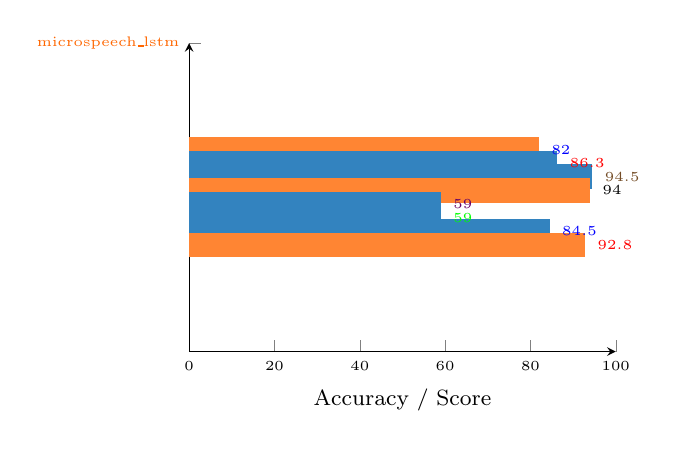
\begin{tikzpicture}
\begin{axis}[
  xbar,
  width=7cm, height=5.5cm,
  bar width=9pt,
  xlabel={\footnotesize Accuracy / Score},
  ytick=data,
  yticklabels={
    \textcolor{NXPOrange}{microspeech\_lstm},
    \textcolor{ADIBlue}{conv1d\_audionet},
    \textcolor{ADIBlue}{ds\_cnn (MAX32690)},
    \textcolor{NXPOrange}{ds\_cnn (i.MX)},
    \textcolor{ADIBlue}{rnnoise (PESQ)},
    \textcolor{ADIBlue}{dtln (PESQ)},
    \textcolor{ADIBlue}{genrenet (genre)},
    \textcolor{NXPOrange}{wav2letter (1-WER)}
  },
  yticklabel style={font=\tiny},
  xticklabel style={font=\tiny},
  xmin=0,xmax=100,
  nodes near coords,
  nodes near coords style={font=\tiny,xshift=1pt},
  axis lines=left,
  tick align=inside,
]
\addplot+[xbar,fill=NXPOrange!80,draw=none] coordinates {(82,7)};
\addplot+[xbar,fill=ADIBlue!80,draw=none] coordinates {(86.3,6)};
\addplot+[xbar,fill=ADIBlue!80,draw=none] coordinates {(94.5,5)};
\addplot+[xbar,fill=NXPOrange!80,draw=none] coordinates {(94.0,4)};
\addplot+[xbar,fill=ADIBlue!80,draw=none] coordinates {(59,3)};
\addplot+[xbar,fill=ADIBlue!80,draw=none] coordinates {(59,2)};
\addplot+[xbar,fill=ADIBlue!80,draw=none] coordinates {(84.5,1)};
\addplot+[xbar,fill=NXPOrange!80,draw=none] coordinates {(92.8,0)};
\end{axis}
\end{tikzpicture}
\column{0.45\textwidth}
\footnotesize
\begin{block}{KWS Comparison}
\begin{tabular}{@{}lll@{}}
\textbf{Model} & \textbf{HW} & \textbf{Acc}\\
\midrule
ds\_cnn & MAX32690 & 94.5\%\\
ds\_cnn & i.MX & 94.0\%\\
conv1d & MAX78002 & 86.3\%\\
microspeech & RT1170 & $\sim$82\%\\
\end{tabular}
\end{block}
\begin{block}{ASR (wav2letter)}
\textcolor{NXPOrange}{\textbf{NXP exclusive}} --- CTC end-to-end ASR\\
WER: \textbf{7.2\%} on LibriSpeech\\
Input: (1, 296, 39) MFCC\\
\textbf{Full sentence recognition} on edge
\end{block}
\begin{block}{Denoising}
PESQ 2.95/5.0 for both RNNoise (ADI)\\
and DTLN (ADI) --- real-time capable
\end{block}
\end{columns}
\end{frame}

% -------------------------------------------------
\begin{frame}{NXP-Exclusive: Image Enhancement \& Biometric Models}
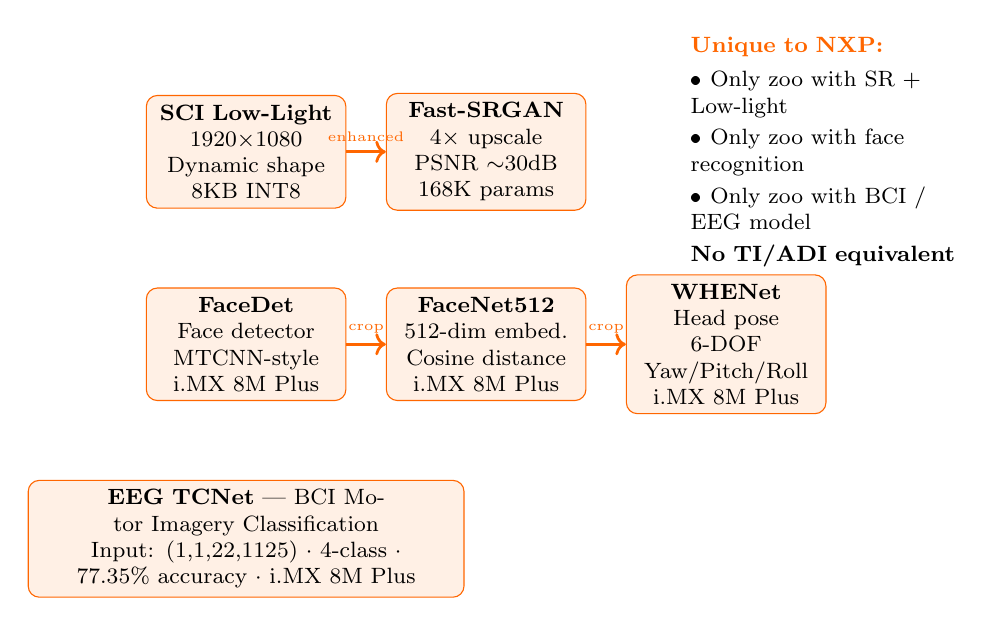
\begin{tikzpicture}[node distance=0.4cm and 0.5cm]
\node[draw=NXPOrange,fill=NXPOrange!10,rounded corners,minimum width=2.5cm,
      minimum height=1.1cm,text width=2.3cm,align=center,font=\footnotesize] (sci)
  {\textbf{SCI Low-Light}\\1920$\times$1080\\Dynamic shape\\8KB INT8};
\node[right=of sci,draw=NXPOrange,fill=NXPOrange!10,rounded corners,
      minimum width=2.5cm,minimum height=1.1cm,text width=2.3cm,align=center,
      font=\footnotesize] (srgan) {\textbf{Fast-SRGAN}\\4$\times$ upscale\\PSNR $\sim$30dB\\168K params};
\draw[->,line width=1pt,NXPOrange] (sci) -- (srgan)
  node[midway,above,font=\tiny]{enhanced};
\node[below=1.0cm of sci,draw=NXPOrange,fill=NXPOrange!10,rounded corners,
      minimum width=2.5cm,minimum height=1.1cm,text width=2.3cm,align=center,
      font=\footnotesize] (facedet)
  {\textbf{FaceDet}\\Face detector\\MTCNN-style\\i.MX 8M Plus};
\node[right=of facedet,draw=NXPOrange,fill=NXPOrange!10,rounded corners,
      minimum width=2.5cm,minimum height=1.1cm,text width=2.3cm,align=center,
      font=\footnotesize] (facenet) {\textbf{FaceNet512}\\512-dim embed.\\Cosine distance\\i.MX 8M Plus};
\node[right=of facenet,draw=NXPOrange,fill=NXPOrange!10,rounded corners,
      minimum width=2.5cm,minimum height=1.1cm,text width=2.3cm,align=center,
      font=\footnotesize] (whenet) {\textbf{WHENet}\\Head pose 6-DOF\\Yaw/Pitch/Roll\\i.MX 8M Plus};
\draw[->,line width=1pt,NXPOrange] (facedet) -- (facenet)
  node[midway,above,font=\tiny]{crop};
\draw[->,line width=1pt,NXPOrange] (facenet) -- (whenet)
  node[midway,above,font=\tiny]{crop};
\node[below=1.0cm of facedet,draw=NXPOrange,fill=NXPOrange!10,rounded corners,
      minimum width=5.5cm,minimum height=1.1cm,text width=5.3cm,align=center,
      font=\footnotesize] (eeg)
  {\textbf{EEG TCNet} --- BCI Motor Imagery Classification\\Input: (1,1,22,1125) $\cdot$ 4-class $\cdot$ 77.35\% accuracy $\cdot$ i.MX 8M Plus};
\node[right=1.2cm of srgan,font=\footnotesize,text width=3.5cm,align=left] {
  \textcolor{NXPOrange}{\textbf{Unique to NXP:}}\\[3pt]
  \textbullet\ Only zoo with SR + Low-light\\[2pt]
  \textbullet\ Only zoo with face recognition\\[2pt]
  \textbullet\ Only zoo with BCI / EEG model\\[2pt]
  \textbf{No TI/ADI equivalent}
};
\end{tikzpicture}
\end{frame}

% ================================================
\section{Quantization Comparison}
% ================================================

\begin{frame}{Quantization Strategy: PTQ vs.\ QAT}
\begin{tikzpicture}[node distance=0.3cm]
\node[draw=TIRed,fill=TIRed!8,rounded corners,minimum width=3.8cm,
      minimum height=4.8cm,text width=3.6cm,align=left,font=\footnotesize,
      inner sep=6pt] (ti) at (0,0) {
  \textcolor{TIRed}{\textbf{TI --- TIDL PTQ}}\\[5pt]
  \textbf{When:} After training\\
  \textbf{Data:} 50--500 frames\\
  \textbf{Bits:} INT8 (16 opt.)\\[5pt]
  \textbf{Drop:} 0.5--2\%\\
  \textbf{Fast:} Yes (hours)\\[5pt]
  \textbf{HW:} TIDL whitelist\\
  \ \ required\\[5pt]
  \textbf{Recovery:} Mixed\\
  \ \ precision layers
};
\node[draw=ADIBlue,fill=ADIBlue!8,rounded corners,minimum width=3.8cm,
      minimum height=4.8cm,text width=3.6cm,align=left,font=\footnotesize,
      inner sep=6pt,right=0.4cm of ti] (adi) {
  \textcolor{ADIBlue}{\textbf{ADI --- AI8X QAT}}\\[5pt]
  \textbf{When:} During training\\
  \textbf{Data:} Full dataset\\
  \textbf{Bits:} INT4/INT8 weights\\
  \ \ INT8 activations\\[5pt]
  \textbf{Drop:} $<$0.5\% (near-lossless)\\
  \textbf{Fast:} No (full retrain)\\[5pt]
  \textbf{HW:} CNN accel.\\
  \ \ op-set constraint\\[5pt]
  \textbf{Recovery:} QAT\\
  \ \ schedule tuning
};
\node[draw=NXPOrange,fill=NXPOrange!8,rounded corners,minimum width=3.8cm,
      minimum height=4.8cm,text width=3.6cm,align=left,font=\footnotesize,
      inner sep=6pt,right=0.4cm of adi] (nxp) {
  \textcolor{NXPOrange}{\textbf{NXP --- TFLite PTQ}}\\[5pt]
  \textbf{When:} After training\\
  \textbf{Data:} 100--1000 samples\\
  \textbf{Bits:} INT8 (per-channel)\\[5pt]
  \textbf{Drop:} 0.5--3\%\\
  \textbf{Fast:} Yes (minutes)\\[5pt]
  \textbf{HW:} TFLite ops +\\
  \ \ Vela for Ethos-U65\\[5pt]
  \textbf{Recovery:} Larger\\
  \ \ calibration set
};
\node[below=0.2cm of adi,font=\tiny\bfseries,text=AccentGreen]
  {\faCheckCircle\ Best accuracy retention};
\node[below=0.2cm of ti,font=\tiny\bfseries,text=TIRed]
  {Fast deployment};
\node[below=0.2cm of nxp,font=\tiny\bfseries,text=NXPOrange]
  {Standard toolchain};
\end{tikzpicture}
\end{frame}

\begin{frame}{Accuracy Drop: FP32 $\rightarrow$ INT8}
\begin{columns}
\column{0.55\textwidth}
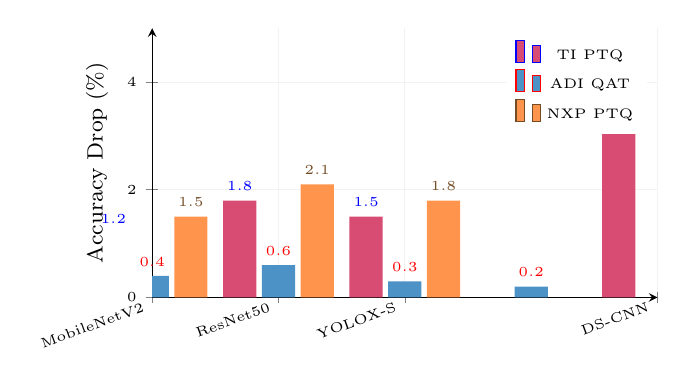
\begin{tikzpicture}
\begin{axis}[
  ybar,
  width=8cm, height=5cm,
  bar width=12pt,
  ylabel={\footnotesize Accuracy Drop (\%)},
  xtick=data,
  xticklabels={MobileNetV2,ResNet50,YOLOX-S,DS-CNN,Swin-Tiny},
  xticklabel style={font=\tiny,rotate=20,anchor=east},
  yticklabel style={font=\tiny},
  ylabel style={font=\tiny},
  ymin=0,ymax=5,
  legend style={font=\tiny,at={(0.98,0.98)},anchor=north east,draw=none},
  grid=major,grid style={gray!10},
  axis lines=left,
  nodes near coords,
  nodes near coords style={font=\tiny},
]
\addplot+[fill=TIRed!70,draw=none] coordinates {(0,1.2)(1,1.8)(2,1.5)(4,4.2)};
\addlegendentry{TI PTQ}
\addplot+[fill=ADIBlue!70,draw=none] coordinates {(0,0.4)(1,0.6)(2,0.3)(3,0.2)};
\addlegendentry{ADI QAT}
\addplot+[fill=NXPOrange!70,draw=none] coordinates {(0,1.5)(1,2.1)(2,1.8)};
\addlegendentry{NXP PTQ}
\end{axis}
\end{tikzpicture}
\column{0.42\textwidth}
\footnotesize
\begin{block}{Analysis}
\begin{itemize}
  \item \textcolor{ADIBlue}{\textbf{ADI QAT}} consistently $<$0.6\% drop --- best quantization quality
  \item \textcolor{TIRed}{\textbf{TI Swin-Tiny}} 4.2\% drop --- transformer architectures harder to quantize
  \item \textcolor{NXPOrange}{\textbf{NXP}} and \textcolor{TIRed}{\textbf{TI}} PTQ comparable for CNNs
\end{itemize}
\end{block}
\begin{alertblock}{Recommendation}
Use \textbf{QAT} for accuracy-critical deployments; PTQ when training re-run is not feasible.
\end{alertblock}
\end{columns}
\end{frame}

% ================================================
\section{Multi-Model Pipelines}
% ================================================

\begin{frame}{TI ADAS Scene Understanding Pipeline}
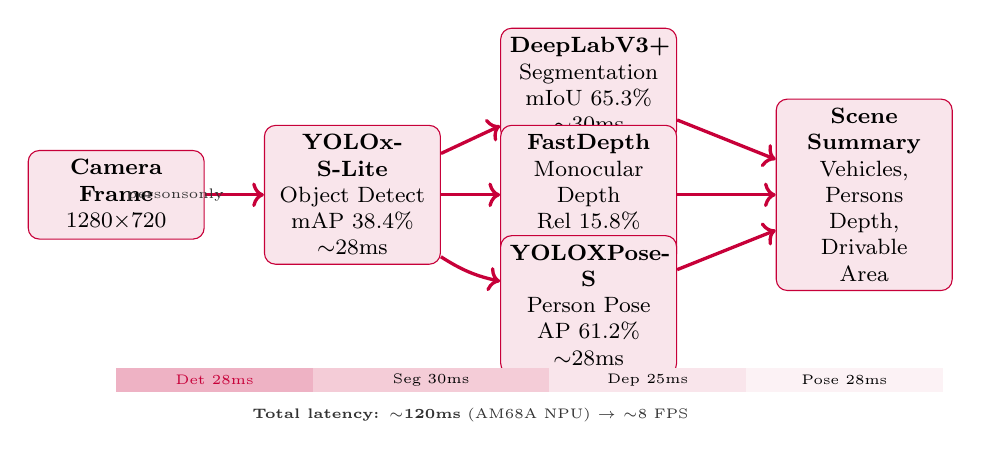
\begin{tikzpicture}[
  box/.style={draw=TIRed,fill=TIRed!10,rounded corners=4pt,
              minimum height=1.1cm,text width=2.0cm,align=center,font=\footnotesize},
  arr/.style={->,line width=1.2pt,TIRed},
  note/.style={font=\tiny,text=DarkGray}
]
\node[box] (input) at (0,0) {\textbf{Camera Frame}\\1280$\times$720};
\node[box] (det) at (3,0) {\textbf{YOLOx-S-Lite}\\Object Detect\\mAP 38.4\%\\$\sim$28ms};
\node[box] (seg) at (6,1.4) {\textbf{DeepLabV3+}\\Segmentation\\mIoU 65.3\%\\$\sim$30ms};
\node[box] (dep) at (6,0) {\textbf{FastDepth}\\Monocular Depth\\Rel 15.8\%\\$\sim$25ms};
\node[box] (pose) at (6,-1.4) {\textbf{YOLOXPose-S}\\Person Pose\\AP 61.2\%\\$\sim$28ms};
\node[box] (fuse) at (9.5,0) {\textbf{Scene Summary}\\Vehicles, Persons\\Depth, Drivable\\Area};
\draw[arr] (input) -- (det);
\draw[arr] (det) -- (seg);
\draw[arr] (det) -- (dep);
\draw[arr] (det) to[bend right=10] (pose) node[midway,note,right]{persons\\only};
\draw[arr] (seg) -- (fuse);
\draw[arr] (dep) -- (fuse);
\draw[arr] (pose) -- (fuse);
\node[note] at (4.5,-2.8) {\textbf{Total latency: $\sim$120ms} (AM68A NPU) $\rightarrow$ $\sim$8 FPS};
\draw[fill=TIRed!30,draw=none] (0,-2.5) rectangle (2.5,-2.2)
  node[midway,font=\tiny]{\textcolor{TIRed}{Det 28ms}};
\draw[fill=TIRed!20,draw=none] (2.5,-2.5) rectangle (5.5,-2.2)
  node[midway,font=\tiny]{Seg 30ms};
\draw[fill=TIRed!10,draw=none] (5.5,-2.5) rectangle (8,-2.2)
  node[midway,font=\tiny]{Dep 25ms};
\draw[fill=TIRed!5,draw=none] (8,-2.5) rectangle (10.5,-2.2)
  node[midway,font=\tiny]{Pose 28ms};
\end{tikzpicture}
\end{frame}

% -------------------------------------------------
\begin{frame}{ADI Smart Sensor Node: Hierarchical Activation}
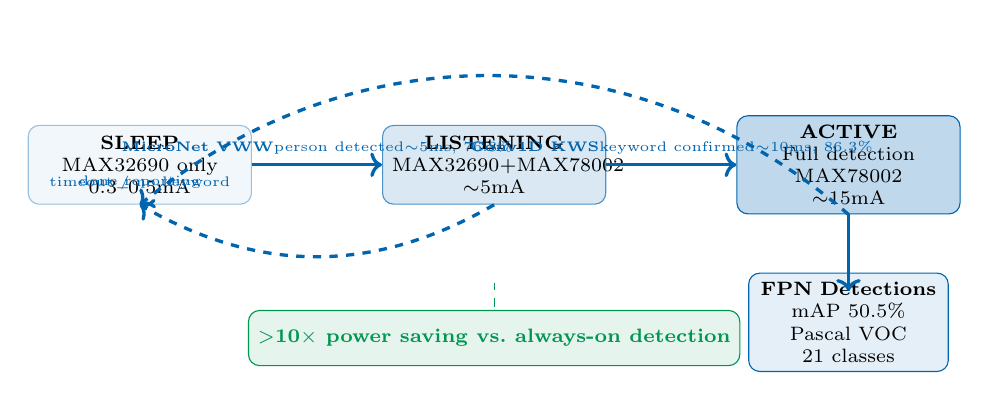
\begin{tikzpicture}[
  box/.style={rounded corners=4pt,minimum height=1.0cm,
              text width=2.6cm,align=center,font=\scriptsize},
  arr/.style={->,line width=1.2pt},
]
\node[draw=ADIBlue!40,fill=ADIBlue!5,box] (sleep) at (0,0)
  {\textbf{SLEEP}\\MAX32690 only\\0.3--0.5mA};
\node[draw=ADIBlue!70,fill=ADIBlue!15,box] (listen) at (4.5,0)
  {\textbf{LISTENING}\\MAX32690+MAX78002\\$\sim$5mA};
\node[draw=ADIBlue,fill=ADIBlue!25,box] (active) at (9,0)
  {\textbf{ACTIVE}\\Full detection\\MAX78002\\$\sim$15mA};
\draw[arr,ADIBlue] (sleep) -- (listen)
  node[midway,above,font=\tiny]{\textbf{MicroNet VWW}\\person detected\\$\sim$5ms, 76.8\%};
\draw[arr,ADIBlue] (listen) -- (active)
  node[midway,above,font=\tiny]{\textbf{Conv1D KWS}\\keyword confirmed\\$\sim$10ms, 86.3\%};
\draw[arr,ADIBlue,dashed] (listen.south) to[bend left=30] (sleep.south)
  node[midway,below,font=\tiny]{timeout / no keyword};
\draw[arr,ADIBlue,dashed] (active.south) to[bend right=40] (sleep.south)
  node[midway,below,font=\tiny]{done reporting};
\node[draw=AccentGreen,fill=AccentGreen!10,rounded corners,
      font=\scriptsize\bfseries,text=AccentGreen,
      minimum width=3cm,minimum height=0.7cm] at (4.5,-2.2)
  {$>$10$\times$ power saving vs.\ always-on detection};
\draw[-,dashed,AccentGreen] (4.5,-1.8) -- (4.5,-1.5);
\node[draw=ADIBlue,fill=ADIBlue!10,rounded corners,font=\scriptsize,
      text width=2.3cm,align=center,minimum height=0.9cm]
  at (9,-2.0) {\textbf{FPN Detections}\\mAP 50.5\%\\Pascal VOC\\21 classes};
\draw[arr,ADIBlue] (active.south) -- (9,-1.6);
\end{tikzpicture}
\end{frame}

% -------------------------------------------------
\begin{frame}{NXP Low-Light Face Recognition Pipeline}
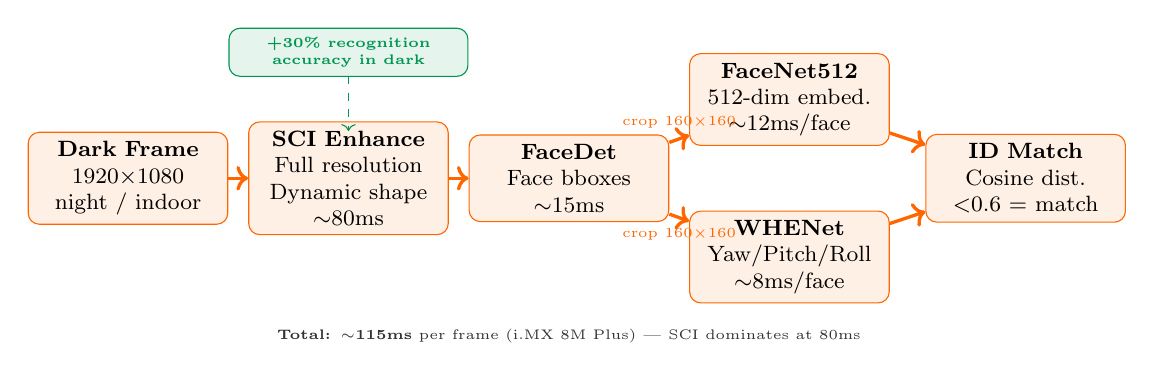
\begin{tikzpicture}[
  box/.style={draw=NXPOrange,fill=NXPOrange!10,rounded corners=4pt,
              minimum height=1.1cm,text width=2.3cm,align=center,font=\footnotesize},
  arr/.style={->,line width=1.2pt,NXPOrange},
]
\node[box] (frame) at (0,0) {\textbf{Dark Frame}\\1920$\times$1080\\night / indoor};
\node[box] (sci) at (2.8,0) {\textbf{SCI Enhance}\\Full resolution\\Dynamic shape\\$\sim$80ms};
\node[box] (fdet) at (5.6,0) {\textbf{FaceDet}\\Face bboxes\\$\sim$15ms};
\node[box] (fn) at (8.4,1.0) {\textbf{FaceNet512}\\512-dim embed.\\$\sim$12ms/face};
\node[box] (whe) at (8.4,-1.0) {\textbf{WHENet}\\Yaw/Pitch/Roll\\$\sim$8ms/face};
\node[box] (match) at (11.4,0) {\textbf{ID Match}\\Cosine dist.\\$<$0.6 = match};
\draw[arr] (frame) -- (sci);
\draw[arr] (sci) -- (fdet);
\draw[arr] (fdet) -- (fn) node[midway,above,font=\tiny]{crop 160$\times$160};
\draw[arr] (fdet) -- (whe) node[midway,below,font=\tiny]{crop 160$\times$160};
\draw[arr] (fn) -- (match);
\draw[arr] (whe) -- (match);
\node[draw=AccentGreen,fill=AccentGreen!10,rounded corners,
      font=\tiny\bfseries,text=AccentGreen,
      text width=2.8cm,align=center,minimum height=0.6cm] at (2.8,1.6)
  {+30\% recognition accuracy in dark};
\draw[->,dashed,AccentGreen] (2.8,1.3) -- (2.8,0.6);
\node[font=\tiny,text=DarkGray] at (5.6,-2.0)
  {\textbf{Total: $\sim$115ms} per frame (i.MX 8M Plus) --- SCI dominates at 80ms};
\end{tikzpicture}
\end{frame}

% -------------------------------------------------
\begin{frame}{All 9 Multi-Model Pipelines: Latency \& Power}
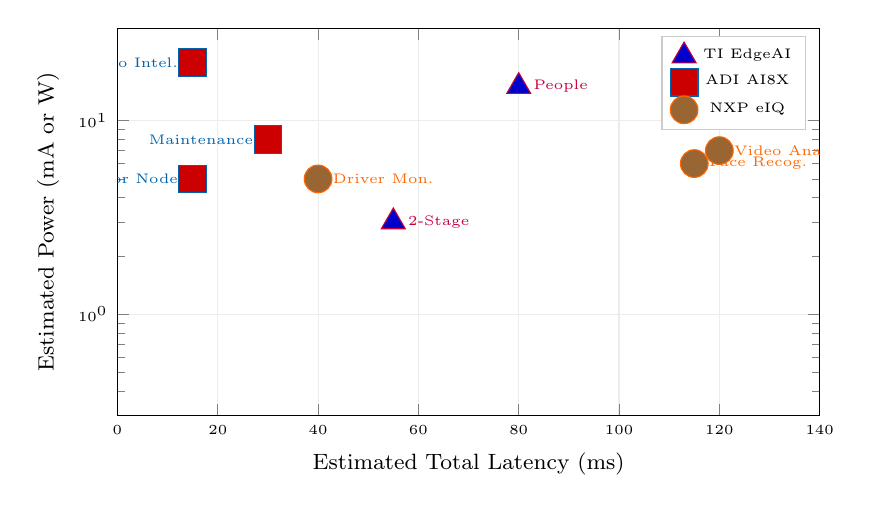
\begin{tikzpicture}
\begin{axis}[
  width=10.5cm, height=6.5cm,
  xlabel={\footnotesize Estimated Total Latency (ms)},
  ylabel={\footnotesize Estimated Power (mA or W)},
  xmin=0, xmax=140,
  ymode=log,
  ymin=0.3, ymax=30,
  grid=major,grid style={gray!15},
  legend style={font=\tiny,at={(0.98,0.98)},anchor=north east,
                draw=gray!40,fill=white},
  xlabel style={font=\tiny},
  ylabel style={font=\tiny},
  xticklabel style={font=\tiny},
  yticklabel style={font=\tiny},
  tick align=inside,
]
\addplot+[only marks,mark=triangle*,mark size=5pt,color=TIRed]
  coordinates {(120,15)(55,3)(80,15)};
\addlegendentry{TI EdgeAI}
\addplot+[only marks,mark=square*,mark size=5pt,color=ADIBlue]
  coordinates {(15,5)(30,8)(15,20)};
\addlegendentry{ADI AI8X}
\addplot+[only marks,mark=*,mark size=5pt,color=NXPOrange]
  coordinates {(115,6)(40,5)(120,7)};
\addlegendentry{NXP eIQ}
\node[font=\tiny,text=TIRed,anchor=west] at (axis cs:121,15) {ADAS};
\node[font=\tiny,text=TIRed,anchor=west] at (axis cs:56,3) {2-Stage};
\node[font=\tiny,text=TIRed,anchor=west] at (axis cs:81,15) {People};
\node[font=\tiny,text=ADIBlue,anchor=east] at (axis cs:14,5) {Sensor Node};
\node[font=\tiny,text=ADIBlue,anchor=east] at (axis cs:29,8) {Maintenance};
\node[font=\tiny,text=ADIBlue,anchor=east] at (axis cs:14,20) {Audio Intel.};
\node[font=\tiny,text=NXPOrange,anchor=west] at (axis cs:116,6) {Face Recog.};
\node[font=\tiny,text=NXPOrange,anchor=west] at (axis cs:41,5) {Driver Mon.};
\node[font=\tiny,text=NXPOrange,anchor=west] at (axis cs:121,7) {Video Anal.};
\end{axis}
\end{tikzpicture}
\end{frame}

% ================================================
\section{Dataset Coverage}
% ================================================

\begin{frame}{Dataset Coverage Matrix}
\small
\begin{tabular}{lcccl}
\toprule
\textbf{Dataset} & \tibox{TI} & \adibox{ADI} & \nxpbox{NXP} & \textbf{Task}\\
\midrule
ImageNet-1K & \textcolor{AccentGreen}{\checkmark} 15 & \textcolor{AccentGreen}{\checkmark} 4 & \textcolor{AccentGreen}{\checkmark} 7 & Classification\\
COCO & \textcolor{AccentGreen}{\checkmark} 11 & \texttimes & \textcolor{AccentGreen}{\checkmark} 5 & Detection\\
Cityscapes & \textcolor{AccentGreen}{\checkmark} 4 & \texttimes & \textcolor{AccentGreen}{\checkmark} 1 & Segmentation\\
Pascal VOC & \texttimes & \textcolor{AccentGreen}{\checkmark} 1 & \texttimes & Detection\\
COCO Keypoints & \textcolor{AccentGreen}{\checkmark} 3 & \texttimes & \textcolor{AccentGreen}{\checkmark} 2 & Pose\\
Google Speech Commands & \texttimes & \textcolor{AccentGreen}{\checkmark} 2 & \textcolor{AccentGreen}{\checkmark} 2 & KWS\\
LibriSpeech & \texttimes & \texttimes & \textcolor{AccentGreen}{\checkmark} 1 & ASR\\
MIMII / DCASE & \texttimes & \textcolor{AccentGreen}{\checkmark} 1 & \textcolor{AccentGreen}{\checkmark} 1 & Anomaly\\
GTZAN & \texttimes & \textcolor{AccentGreen}{\checkmark} 1 & \texttimes & Audio Genre\\
Set5 / Set14 (PSNR) & \texttimes & \texttimes & \textcolor{AccentGreen}{\checkmark} 1 & Super-Res.\\
FaceNet / LFW & \texttimes & \texttimes & \textcolor{AccentGreen}{\checkmark} 1 & Face Recog.\\
BCI Competition IV & \texttimes & \texttimes & \textcolor{AccentGreen}{\checkmark} 1 & EEG / BCI\\
\midrule
\textbf{Datasets covered} & \textbf{5} & \textbf{6} & \textbf{12} & \\
\bottomrule
\end{tabular}
\vspace{0.4cm}
\footnotesize
\textcolor{NXPOrange}{\textbf{NXP}} covers the most datasets (12), including exclusive medical/BCI and image restoration benchmarks.
\end{frame}

% ================================================
\section{Deployment \& MLOps}
% ================================================

\begin{frame}{Deployment Workflow Comparison}
\begin{tikzpicture}[
  step/.style={rounded corners=3pt,minimum height=0.75cm,
               text width=2.1cm,align=center,font=\tiny},
]
\node[font=\small\bfseries,text=TIRed] at (1.6,3.4) {TI EdgeAI};
\node[font=\small\bfseries,text=ADIBlue] at (5.0,3.4) {ADI AI8X};
\node[font=\small\bfseries,text=NXPOrange] at (8.4,3.4) {NXP eIQ};
\foreach \y/\lbl in {3.0/Train, 2.2/Quantize, 1.4/Compile, 0.6/Evaluate, -0.2/Package, -1.0/Deploy}{
  \node[font=\tiny\bfseries,text=DarkGray] at (-0.5,\y) {\lbl};
  \draw[dashed,gray!30] (-0.1,\y) -- (10.1,\y);
}
\node[step,draw=TIRed,fill=TIRed!10] at (1.6,3.0) {ONNX/TFLite\\training};
\node[step,draw=TIRed,fill=TIRed!10] at (1.6,2.2) {TIDL PTQ\\50--500 frames};
\node[step,draw=TIRed,fill=TIRed!10] at (1.6,1.4) {TIDL compile\\.bin artifacts};
\node[step,draw=TIRed,fill=TIRed!10] at (1.6,0.6) {Accuracy gate\\per SoC};
\node[step,draw=TIRed,fill=TIRed!10] at (1.6,-0.2) {.tar.gz bundle};
\node[step,draw=TIRed,fill=TIRed!10] at (1.6,-1.0) {SCP to EVM\\/ OTA};
\node[step,draw=ADIBlue,fill=ADIBlue!10] at (5.0,3.0) {PyTorch QAT\\(ai8x-training)};
\node[step,draw=ADIBlue,fill=ADIBlue!10] at (5.0,2.2) {INT4/INT8\\baked in training};
\node[step,draw=ADIBlue,fill=ADIBlue!10] at (5.0,1.4) {ai8xize.py\\C headers};
\node[step,draw=ADIBlue,fill=ADIBlue!10] at (5.0,0.6) {Accuracy gate\\per device};
\node[step,draw=ADIBlue,fill=ADIBlue!10] at (5.0,-0.2) {.tar.gz bundle\\+ C headers};
\node[step,draw=ADIBlue,fill=ADIBlue!10] at (5.0,-1.0) {Flash to\\MAX78002};
\node[step,draw=NXPOrange,fill=NXPOrange!10] at (8.4,3.0) {recipe.sh\\Docker build};
\node[step,draw=NXPOrange,fill=NXPOrange!10] at (8.4,2.2) {TFLite PTQ\\100--1k samples};
\node[step,draw=NXPOrange,fill=NXPOrange!10] at (8.4,1.4) {Vela compile\\(i.MX 93 only)};
\node[step,draw=NXPOrange,fill=NXPOrange!10] at (8.4,0.6) {PSNR/WER/Acc\\gate};
\node[step,draw=NXPOrange,fill=NXPOrange!10] at (8.4,-0.2) {.tgz + Vela\\+ manifest};
\node[step,draw=NXPOrange,fill=NXPOrange!10] at (8.4,-1.0) {SCP to i.MX\\board};
\end{tikzpicture}
\end{frame}

% -------------------------------------------------
\begin{frame}{MLOps Stack: Shared Architecture}
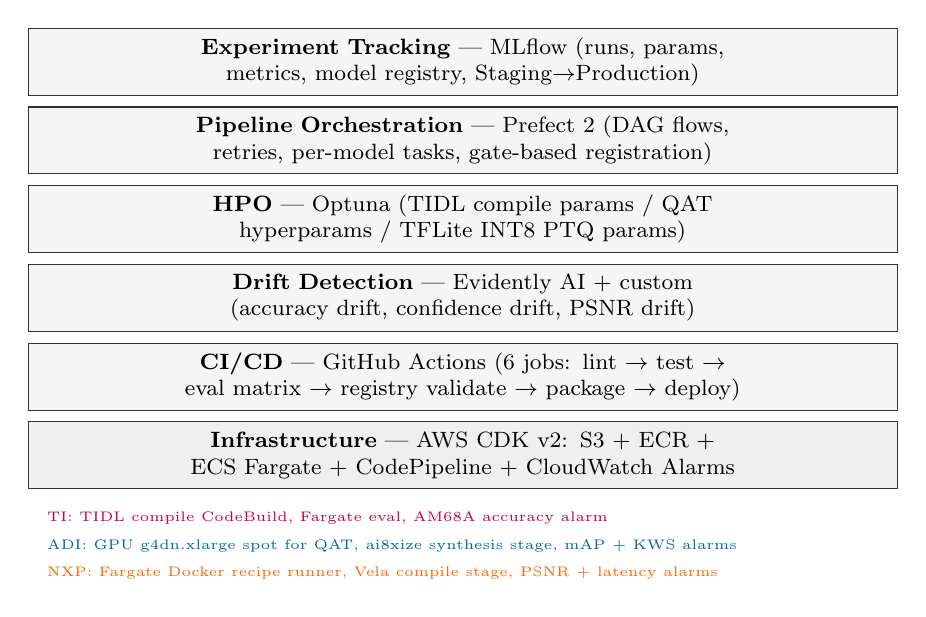
\begin{tikzpicture}[
  layer/.style={minimum width=11cm,minimum height=0.85cm,
                text width=10.8cm,align=center,font=\footnotesize},
]
\node[layer,draw=DarkGray,fill=DarkGray!5] at (5.5,4.0)
  {\textbf{Experiment Tracking} --- MLflow (runs, params, metrics, model registry, Staging$\rightarrow$Production)};
\node[layer,draw=DarkGray,fill=DarkGray!5] at (5.5,3.0)
  {\textbf{Pipeline Orchestration} --- Prefect 2 (DAG flows, retries, per-model tasks, gate-based registration)};
\node[layer,draw=DarkGray,fill=DarkGray!5] at (5.5,2.0)
  {\textbf{HPO} --- Optuna (TIDL compile params / QAT hyperparams / TFLite INT8 PTQ params)};
\node[layer,draw=DarkGray,fill=DarkGray!5] at (5.5,1.0)
  {\textbf{Drift Detection} --- Evidently AI + custom (accuracy drift, confidence drift, PSNR drift)};
\node[layer,draw=DarkGray,fill=DarkGray!5] at (5.5,0.0)
  {\textbf{CI/CD} --- GitHub Actions (6 jobs: lint $\rightarrow$ test $\rightarrow$ eval matrix $\rightarrow$ registry validate $\rightarrow$ package $\rightarrow$ deploy)};
\node[layer,draw=DarkGray,fill=DarkGray!8] at (5.5,-1.0)
  {\textbf{Infrastructure} --- AWS CDK v2: S3 + ECR + ECS Fargate + CodePipeline + CloudWatch Alarms};
\node[font=\tiny,text=TIRed,anchor=west] at (0.1,-1.8)
  {TI: TIDL compile CodeBuild, Fargate eval, AM68A accuracy alarm};
\node[font=\tiny,text=ADIBlue,anchor=west] at (0.1,-2.15)
  {ADI: GPU g4dn.xlarge spot for QAT, ai8xize synthesis stage, mAP + KWS alarms};
\node[font=\tiny,text=NXPOrange,anchor=west] at (0.1,-2.5)
  {NXP: Fargate Docker recipe runner, Vela compile stage, PSNR + latency alarms};
\end{tikzpicture}
\end{frame}

% ================================================
\section{Tradeoffs \& Recommendations}
% ================================================

\begin{frame}{Key Tradeoffs: Accuracy vs.\ Power vs.\ Flexibility}
\begin{columns}
\column{0.58\textwidth}
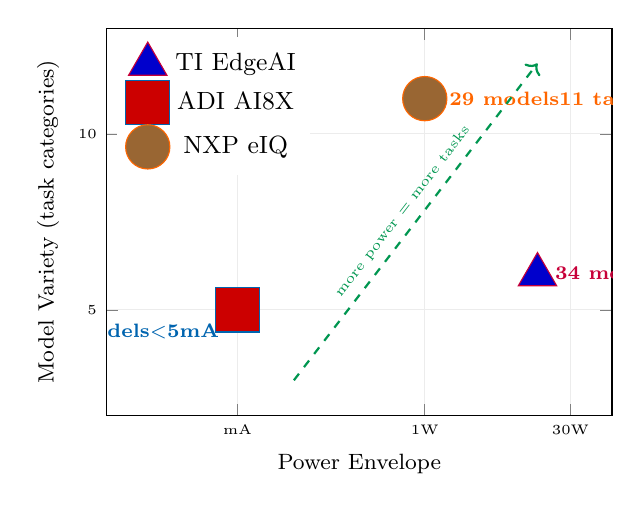
\begin{tikzpicture}
\begin{axis}[
  width=8cm,height=6.5cm,
  xlabel={\footnotesize Power Envelope},
  ylabel={\footnotesize Model Variety (task categories)},
  xmode=log,
  xmin=0.1,xmax=50,
  ymin=2,ymax=13,
  grid=major,grid style={gray!15},
  legend style={font=\small,at={(0.02,0.98)},anchor=north west,draw=none},
  xlabel style={font=\tiny},
  ylabel style={font=\tiny},
  xticklabel style={font=\tiny},
  yticklabel style={font=\tiny},
  xtick={0.5,5,30},
  xticklabels={mA,1W,30W},
]
\addplot+[only marks,mark=triangle*,mark size=8pt,color=TIRed,draw=TIRed]
  coordinates {(20,6)};
\addlegendentry{TI EdgeAI}
\addplot+[only marks,mark=square*,mark size=8pt,color=ADIBlue,draw=ADIBlue]
  coordinates {(0.5,5)};
\addlegendentry{ADI AI8X}
\addplot+[only marks,mark=*,mark size=8pt,color=NXPOrange,draw=NXPOrange]
  coordinates {(5,11)};
\addlegendentry{NXP eIQ}
\node[font=\scriptsize\bfseries,text=TIRed,anchor=west] at (axis cs:22,6)
  {34 models / 5 SoCs\\ADAS-grade};
\node[font=\scriptsize\bfseries,text=ADIBlue,anchor=east] at (axis cs:0.45,4.4)
  {15 models\\$<$5mA};
\node[font=\scriptsize\bfseries,text=NXPOrange,anchor=west] at (axis cs:6,11)
  {29 models\\11 tasks};
\draw[->,AccentGreen,dashed,line width=0.8pt] (axis cs:1,3) -- (axis cs:20,12)
  node[midway,font=\tiny,sloped,above,text=AccentGreen]{more power = more tasks};
\end{axis}
\end{tikzpicture}
\column{0.39\textwidth}
\footnotesize
\begin{block}{Choose \textcolor{TIRed}{TI} when:}
\begin{itemize}
  \item Automotive SoC (TDA4VM)
  \item Highest det. accuracy (rtmdet 60\%)
  \item ISO 26262 ASIL-B required
\end{itemize}
\end{block}
\begin{block}{Choose \textcolor{ADIBlue}{ADI} when:}
\begin{itemize}
  \item Battery life critical ($<$5mA)
  \item QAT quality required
  \item Motor fault detection
\end{itemize}
\end{block}
\begin{block}{Choose \textcolor{NXPOrange}{NXP} when:}
\begin{itemize}
  \item Widest task coverage needed
  \item Face / SR / BCI required
  \item Linux + MCU range
\end{itemize}
\end{block}
\end{columns}
\end{frame}

% -------------------------------------------------
\begin{frame}{Summary Scorecard}
\begin{center}
\small
\begin{tabular}{lccc}
\toprule
\textbf{Criterion} & \tibox{TI EdgeAI} & \adibox{ADI AI8X} & \nxpbox{NXP eIQ}\\
\midrule
Model variety & $\bigstar\bigstar\bigstar\bigstar\bigstar$ & $\bigstar\bigstar\bigstar$ & $\bigstar\bigstar\bigstar\bigstar$\\
Classification accuracy & $\bigstar\bigstar\bigstar\bigstar\bigstar$ & $\bigstar\bigstar\bigstar$ & $\bigstar\bigstar\bigstar\bigstar$\\
Detection accuracy & $\bigstar\bigstar\bigstar\bigstar\bigstar$ & $\bigstar\bigstar\bigstar\bigstar$ & $\bigstar\bigstar\bigstar\bigstar$\\
Audio support & $\bigstar$ & $\bigstar\bigstar\bigstar\bigstar$ & $\bigstar\bigstar\bigstar\bigstar$\\
Power efficiency & $\bigstar\bigstar$ & $\bigstar\bigstar\bigstar\bigstar\bigstar$ & $\bigstar\bigstar\bigstar$\\
Quantization quality & $\bigstar\bigstar\bigstar$ & $\bigstar\bigstar\bigstar\bigstar\bigstar$ & $\bigstar\bigstar\bigstar$\\
Task diversity & $\bigstar\bigstar\bigstar$ & $\bigstar\bigstar\bigstar$ & $\bigstar\bigstar\bigstar\bigstar\bigstar$\\
Deployment simplicity & $\bigstar\bigstar\bigstar$ & $\bigstar\bigstar$ & $\bigstar\bigstar\bigstar\bigstar$\\
Multi-model pipelines & $\bigstar\bigstar\bigstar\bigstar\bigstar$ & $\bigstar\bigstar\bigstar\bigstar$ & $\bigstar\bigstar\bigstar\bigstar\bigstar$\\
MLOps maturity & $\bigstar\bigstar\bigstar\bigstar$ & $\bigstar\bigstar\bigstar\bigstar$ & $\bigstar\bigstar\bigstar\bigstar$\\
Unique capabilities & ADAS suite & Ultra-LP/QAT & SR+BCI+Face\\
\midrule
\textbf{Best for} & \textbf{Automotive} & \textbf{Battery IoT} & \textbf{Consumer/Ind.}\\
\bottomrule
\end{tabular}
\end{center}
\end{frame}

% -------------------------------------------------
\begin{frame}{Conclusion}
\begin{columns}
\column{0.48\textwidth}
\begin{block}{\textcolor{TIRed}{\faCheckCircle}\ TI EdgeAI --- Key Strengths}
\begin{itemize}
  \item \textbf{34 models}, 5 SoCs --- widest vision portfolio
  \item Highest classification accuracy (\textbf{81.2\%}) and detection mAP (\textbf{60\%})
  \item ADAS-grade hardware (ISO 26262)
  \item Best 4-stage pipeline capability
\end{itemize}
\end{block}
\begin{block}{\textcolor{ADIBlue}{\faCheckCircle}\ ADI AI8X --- Key Strengths}
\begin{itemize}
  \item \textbf{Ultra-low power} (0.3--5mA)
  \item \textbf{QAT} --- near-lossless quantization
  \item Multi-modal: vision + audio + vibration
  \item Hierarchical wake saves \textbf{$>$10$\times$} power
\end{itemize}
\end{block}
\column{0.48\textwidth}
\begin{block}{\textcolor{NXPOrange}{\faCheckCircle}\ NXP eIQ --- Key Strengths}
\begin{itemize}
  \item \textbf{11 task categories} --- broadest coverage
  \item \textbf{Exclusive}: SR, low-light, face recog., BCI
  \item TFLite standard --- simplest deployment
  \item i.MX 8M Plus NPU + Vela for i.MX 93
\end{itemize}
\end{block}
\vspace{0.3cm}
\begin{alertblock}{Bottom Line}
\footnotesize
No single zoo dominates all criteria. Choose based on:
\textbf{power budget} (ADI $\ll$ NXP $\ll$ TI),
\textbf{task needs} (audio/SR/BCI $\rightarrow$ NXP; pure ADAS $\rightarrow$ TI),
\textbf{quantization approach} (QAT accuracy $\rightarrow$ ADI).
\end{alertblock}
\end{columns}
\end{frame}

\end{document}
